\section{Zielsetzung}

    \noindent In diesem Versuch werden Dipole in dotierten Ionenkristallen näher betrachtet. Dabei sollen die Aktivierungsenergie $W$ und die charakteristische Relaxationszeit $\tau_0$ 
    des hier benutzten Kaliumbromid ermittelt werden. 


\section{Theorie}
\label{sec:Theorie}

    \noindent Ein Ionenkristall ist ein Festkörper aus Kationen und Anionen, welche regelmäßig auf einem Gitter angeordnet sind. Die Anordnung wird durch die Ionenbindung zusammengehalten. 

    \subsection{Dipole im dotierte Ionenkristall}

        \noindent Die im Versuch benutzte Probe besteht aus Kalium-Kationen und Bromid-Anionen, welche wie in der \autoref{fig:KBr} auf einem einfachen Gitter angeordnet sind. 
        Kalium ist ein Alkalimetall, die Kalium-Kationen sind also einfach positiv geladen, Brom ist ein Halogen, die Bromid-Anionen also einfach negativ geladen. 
        Nun kann ein Ionenkristall dotiert werden, es werden Ionen eines anderen Stoffes in das Gitter eingebaut. Der Kaliumbromidkristall wird mit Strontium dotiert. Ein einfach 
        positives Kalium-Kation wird durch ein zweifach positives Strontium-Kation ($\ce{Sr^{2+}}$) ersetzt. Damit im Kristall insgesamt noch Ladungsneutralität herrscht, wird ein anderes 
        Kalium-Kation ausgestoßen, sodass im Kristall eine Leerstelle ausgebildet wird. Diese Kombination aus zweifach positiv geladenem Strontium-Ion und der Leerstelle stellt einen 
        Dipol im Ionenkristall dar. Bei Raumtemperatur sind die Dipole statistisch verteilt, sodass das Gesamtdipolmoment des Kristalls verschwindet.

        \begin{figure}[h]
            \centering
            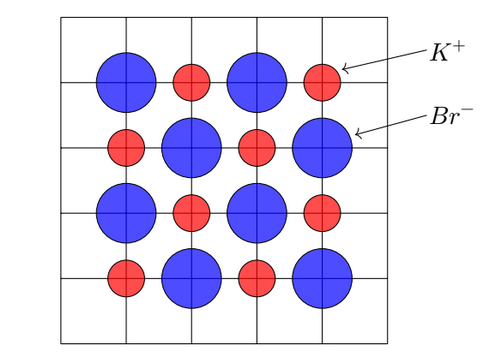
\includegraphics[width=0.4\textwidth]{bilder/Kaliumbromid.png}
            \caption{Eine schematische Abbildung des Kaliumbromid-Ionenkristalls.}
            \label{fig:KBr}
        \end{figure}

        \noindent Der Dipol kann im Ionenkristall nur diskrete Dipolrichtungen einnehmen, da die Leerstelle einen Gitterplatz einnehmen muss. In einem Temperaturbereich von unter 
        $\SI{500}{\celsius}$ kann der Dipol nur unter Leerstellendiffusion seine Richtung ändern. Die dafür benötigte Energie $W$ ist die materialspezifische Aktivierungsenergie.  
        Durch die Boltzmann-Statistik ist der Anteil der Dipole beschrieben, die diese Energie $W$ durch thermische Bewegung aufbringen können, also es gilt $\exp\left(- \frac{W}{k_\text{B}T}\right)$.
        Die Zeit, in welcher sich der Dipol seinem Ausgangszustand nähert, wird Relaxationszeit genannt. Es gilt der Zusammenhang
        \begin{equation*}
            \tau(T) = \tau_0 \cdot \exp \left(\frac{W}{k_\text{B}T}\right)\, ,
        \end{equation*}
        wobei $\tau_0 = \tau(\infty)$ die charakteristische Relaxationszeit eines spezifischen Stoffes ist. 


    \subsection{Depolarisationsstrom}

        \noindent In diesem Versuch werden die Dipole im Kristall ausgerichtet und in diesem Zustand eingefroren. Beim Erwärmen der Probe wird ein Strom gemessen, welcher aufgrund der 
        Reorientierung der Dipole zurück in ihre Ausgangslage existiert. Dieser Depolarisationsstrom kann über zwei verschiedene Ansätze hergeleitet werden. \\

        \noindent Bei dem Polarisationsansatz wird der Depolarisationsstrom im Allgemeinen betrachtet, also 
        \begin{equation}
            I(T) = - \frac{\text{d} P(t)}{\text{d}t} \,.
            \label{eqn:polansa1}
        \end{equation}
        Die zeitliche Änderung der Polarisation ist von der Polarisation zum Zeitpunkt $t$ und von der Relaxationszeit $\tau(T)$ ab
        \begin{equation}
            \frac{\text{d} P(t)}{\text{d}t} = - \frac{P(t)}{\tau(T)} \, ,
            \label{eqn:polansa2}
        \end{equation}
        eingesetzt in die Gleichung \eqref{eqn:polansa1} ergibt 
        sich
        \begin{equation}
            I(T) = \frac{P(t)}{\tau(T)}.
            \label{eqn:polansa3}
        \end{equation}
        Die Gleichung \eqref{eqn:polansa2} ist eine Differetialgleichung für die Polarisation $P(t)$, welche durch einfache Integration gelöst werden kann:
        \begin{equation}
            P(t) = P_0 \exp\left(- \frac{t}{\tau(T)}\right)
            \label{eqn:polansa4}
        \end{equation}
        Die Zeit $t$ gibt die Zeit an, welche benötigt wird um die Temperatur $T$ zu erreichen, somit kann dies auch als Integral geschrieben werden 
        \begin{equation}
            I(T) = \frac{P_0}{\tau(T)} \exp\left( - \frac{t}{\tau(T)}\right) = \frac{P_0}{\tau(T)} \exp\left( - \int_0^t\frac{\text{d}t}{\tau(T)}\right)\, . 
            \label{eqn:polansa5}
        \end{equation}
        Wenn eine konstante Heizrate $b$ vorausgesetzt wird 
        \begin{equation}
            b \coloneq \frac{\text{d}T}{\text{d}t} = \text{const}\, , 
            \label{eqn:heizrate1}
        \end{equation}
        ergibt letztendlich für den Depolarisationsstrom
        \begin{equation}
            I(T) = \frac{P_0}{\tau(T)} \exp\left( - \frac{1}{b}\int_{T_0}^T\frac{\text{d}T'}{\tau(T')}\right)\, .
        \end{equation}

        \noindent Ein weiterer Ansatz um den Depolarisationsstrom herzuleiten ergibt sich durch Betrachtung der Stromdichte. Wird ein Dipol einem externen 
        elektrischen Feld ausgesetzt, dann richtet sich der Teil $y(t)$ der Dipole, welcher durch die Langevin Funktion gegeben ist, in Richtung des Feldes aus.
        Unter der Annahme, dass $pE \ll k_{\text{B}} T$ mit dem Dipolmoment $p$ und dem elektrischen Feld $E$, lässt sich nähern:
        \begin{equation}
            y(t) = \frac{pE}{3 k_\text{B} T}
        \end{equation}
        Wird die konstante Heizrate $b$ aus der Gleichung \eqref{eqn:heizrate1} angelegt, so fließt ein Strom mit der Dichte 
        \begin{equation}
            j(T) = y(T_0) \cdot p \cdot \frac{\text{d}N}{\text{d}t}\, ,
        \end{equation}
        wobei hier $y(T_0)$ der Anteil der Dipole ist, welcher beim Start der Kühlung ausgerichtet sind. Das Differential der Anzahl $N$ bezeichnet die Rate, mit 
        der die Dipole relaxieren. Mit der Annahme, dass die Rate proportional ist, zur Anzahl der noch nicht relaxierten Dipole ist, lässt sich schreiben:
        \begin{equation}
            \frac{\text{d}N(T) }{\text{d} t} = - \frac{N}{\tau(T)}
            \label{eqn:stromdansa1}
        \end{equation}
        Die Lösung der Differentialgleichung ist gegeben durch 
        \begin{equation}
            N = N_0 \exp\left(- \frac{1}{b} \int_{T_0}^{T} \frac{\text{d}T'}{\tau(T')}\right) \, .
        \end{equation}
        Die Konstante $N_0$ bezeichnet die Anzahl der ausgerichteten Dipole vor der Kühlung. Die Stromdichte ist dann insgesamt gegeben durch:
        \begin{equation}
            j(T) = \frac{p^2E}{3 k_\text{B} T} \frac{N_0}{\tau_0} \exp\left(- \frac{1}{b\cdot \tau_0} \int_{T_0}^{T} \exp\left(- \frac{W}{k_\text{B} T'}\right)\,\text{d}T'\right)\cdot  \exp\left(- \frac{W}{k_\text{B} T}\right)
            \label{eqn:Strom2}
        \end{equation}
        % \begin{equation}
            % P_\text{D}(T) = \frac{N}{N_V} \frac{p^2E}{3 k_\text{B} T}\, ,
            % \label{eqn:debye}
        % \end{equation}
        % wobei hier $p$ das Dipolmoment ist, $E$ die elektrische Feldstärke, $T$ die Temperatur, $N_V$ die Dipoldichte und $N$ die Anzahl der Dipole ist. Die 
        % Änderung der Anzahl an Dipole kann über die Relaxationszeit ausgedrückt werden:
        % \begin{equation}
            % \frac{\text{d}N(T) }{\text{d} t} = - \frac{N}{\tau(T)}
            % \label{eqn:stromdansa1}
        % \end{equation}
        % Die Differentialgleichung \eqref{eqn:stromdansa1} wird wieder durch Integration zu 
        % \begin{equation}
            % N = N_0 \exp\left(- \frac{1}{b} \int_{T_0}^{T} \frac{\text{d}T'}{\tau(T')}\right)
        % \end{equation}
        % gelöst. Weiterhin gilt 
        % \begin{align*}
            % I(T) = P_\text{D}(T) \frac{\text{d}N}{\text{d} t} & & \text{und} & & I(T) = - P_\text{D}(T) \frac{N}{\tau(T)}\, .
        % \end{align*}
        % Nach Zusammensetzung aller Terme wird als Ausdruck für den Depolarisationsstrom 
        % \begin{equation}
            % I(T) = \frac{p^2E}{3 k_\text{B} T} \frac{N_0}{N_V \cdot \tau_0} \exp\left(- \frac{1}{b\cdot \tau_0} \int_{T_0}^{T} \exp\left(- \frac{W}{k_\text{B} T'}\right)\,\text{d}T'\right)\cdot  \exp\left(- \frac{W}{k_\text{B} T}\right)
            % \label{eqn:Strom2}
        % \end{equation}
        % erhalten.


    \subsection{Berechnung der Aktivierungsenergie}

        \noindent Die Eigenschaften des dotierten Ionenkristalles, welche in diesem Versuch untersucht werden sollen, ist unter anderen die materialspezifische Aktivierungsenergie $W$.
        Diese kann auf zwei verschiedene Wege ermittelt werden.\\
        
        \noindent Im ersten Verfahren wird das Integral in der Gleichung \eqref{eqn:Strom2} näherungsweise gleich null gesetzt:
        \begin{equation*}
            \int_{T_0}^{T} \exp\left(- \frac{W}{k_\text{B} T'}\right)\,\text{d}T' \approx 0
        \end{equation*}
        Damit lässt sich der Strom wie folgt schreiben
        \begin{equation*}
            I(T) \approx \frac{p^2E}{3 k_\text{B} T} \frac{N_0}{ \tau_0} \cdot  \exp\left(- \frac{W}{k_\text{B} T}\right) \,.
        \end{equation*}
        Durch die Anwendung des natürlichen Logarithmus ergibt sich eine Geradengleichung für $\ln\left(I(T)\right)$ gegen $\frac{1}{T}$:
        \begin{equation}
            \ln\left(I(T)\right) = \underbrace{\left(\frac{p^2E}{3 k_\text{B} T} \frac{N_0}{\tau_0}\right)}_{\text{const.}} - \underbrace{\frac{W}{k_\text{B}}}_{\text{Steigung}} \frac{1}{T}
            \label{eqn:geradengleichung}
        \end{equation}
        Die Aktivierungsenergie $W$ errechnet sich also zu 
        \begin{equation*}
            W = m \cdot k_\text{B} \, ,
        \end{equation*}
        wobei $m$ die Steigung der Gerade ist. \\

        \noindent Bei dem zweiten Verfahren wird der gesamte Kurvenverlauf genutzt. Für die Gesamtpolarisation gilt 
        \begin{equation*}
            \frac{\text{d}P}{\text{d}t} = -\frac{P(t)}{\tau(T)}\, .
        \end{equation*}
        Nach dem Umstellen und der Erweiterung mit $\frac{\text{d}T}{\text{d}T}$ wird der Term zu 
        \begin{equation*}
            \tau(T) = P(T) \cdot \frac{\text{d}T}{\frac{\text{d}P}{\text{d}t}\text{d}T } =  \frac{P(t)}{b} \frac{\text{d}T}{\text{d}P}\, ,
        \end{equation*}
        wobei im zweiten Umformungsschritt die Heizrate $b$ eingesetzt wird, welche in der Gleichung \eqref{eqn:heizrate1} eingeführt wird. 
        Nun wird mit $\frac{\text{d}t}{\text{d}t}$ erweitert, sodass sich folgender Term ergibt:
        \begin{equation*}
            \tau(T) = \frac{P(t)}{b} \frac{\frac{\text{d}T}{\text{d}t}}{\frac{\text{d}P}{\text{d}t}}
        \end{equation*}
        Der Ausdruck für die Relaxationszeit kann umgeformt werden, wenn eingesetzt wird, dass die zeitliche Änderung der Polarisation dem Strom entspricht \eqref{eqn:polansa1} 
        und die Polarisation $P$ als $\int \, \text{d}P$ geschrieben werden kann. 
        \begin{equation*}
            \tau(T) = \frac{\int \frac{\text{d}P}{\text{d}t} \text{d}T}{I(T) \cdot b} = \frac{\int_0^\infty I(T') \, \text{d}T'}{I(T) \cdot b}
        \end{equation*}
        Nun wird für die Relaxationszeit eingesetzt und die Gleichung zur Aktivierungsenergie $W$ umgestellt, sodass sich
        \begin{equation}
            W = k_\text{B} T \cdot \ln\left( \frac{\int_0^\infty I(T') \, \text{d}T'}{b \tau_0 \cdot I(T)}\right)
        \end{equation}
        ergibt. Die obere Grenze wird auf $T^*$ gesetzt, wobei $I(T^*) \approx 0$ ist. 


    \subsection{Berechnung der charakteristischen Relaxationszeit}

        \noindent Am Maximalwert der Stromstärke $I$ bei der Temperatur $T_\text{max}$ ist die Ableitung der Stromstärke gleich null. Um die charakteristische Relaxationszeit zu bestimmen
        wird also die Gleichung \eqref{eqn:Strom2} abgeleitet. Es ergibt sich folgende Proportionalität:
        \begin{equation}
            \frac{\text{d}I}{\text{d}T} \propto \frac{1}{\tau_0} \left(- \frac{1}{b \tau_0} \int_{T_0}^T \exp\left(\frac{W}{k_\text{B} T'}\right) \, \text{d}T' - \frac{W}{k_\text{B} T}\right) \cdot \left( \frac{W}{k_\text{B}T^2} - \frac{1}{b\tau_0}\exp\left(- \frac{W}{k_\text{B} T}\right)\right)
            \label{eqn:relaxa}
        \end{equation}
        Für die Relaxationszeit gilt am Maximum 
        \begin{equation}
            \tau_{\text{max}} (T_{\text{max}}) = \frac{k_\text{B} T^2_{\text{max}}}{b W}\, ,
        \end{equation}
        woraus die charakteristische Relaxationszeit $\tau_0$ berechnent werden kann, wenn $\tau_{\text{max}} (T_{\text{max}})$ und $T_{\text{max}}$ in Gleichung \eqref{eqn:relaxa} eingesetzt wird.